
\chapter{HERO Architecture Simulation}
\label{chap:results}

To assess the performance of the HERO architecture a cycle accuracte simulation
enviornment was implemented using SystemC and python. The enviornment was used
to assess the architecture on real networks implemented in pytorch from the TIMM
library. The simulator is composed of two parts. 1) A python based frontend that
can analyse the performance results of any pytorch network on a configuration of
HERO. 2) A SystemC based backend for cycle accurate simulations of HERO running
convolution layers. In this chapter we will first discuss the simulation
enviornment and it's components in \autoref{chap:hero:sim_platform}. The results
from simulating all 695 networks from TIMM using a small HERO instance are given
\autoref{chap:hero:results}.

\section{Simulation Enviornment}
\label{chap:hero:sim_platform}

\subsection{Python Frontend}
\label{chap:hero:sim_platform:frontend}

The python frontend depicted in \autoref{fig:frontend}, expects a list of pytorch models and a dictionary defining the
configuration of a HERO instance as inputs. The configuration specifies the unroll factors
for F, C, the list of kernels sizes supported in direct mode, and the on-chip
storage dedicated for input and output featurmape reuse. The output of the
frontend is a pandas dataframe containing the results from the backend
simulation of the network(s) on the specified hero instance.  
After the frontend
recieves the list of pytorch models, CIGAR extracts the dimensions of all
supported layers (Conv2D and Linear). Afterwhich two layer transformation
operations are performed. The first converts convolution layers that are
unsupported directly into equivelent (1, 1) convolutions as described in
\autoref{chap:dda:dataflow_dse:indirect_mode}. Additionally, linear layers are
reinterpreted as (1, 1) convolutions based on the proof derived from
\autoref{chap:dda:dataflow_dse:indirect_mode:conv_gemm_equiv:proof}. To
determine what layers are supported directly the HERO arch. config being
evaluated is used. After all layers have been converted to equivelent layers
that are supported by HERO, a layer decomposition step is performed to
decompose layers that have featuremaps that are two large to fit in the
HERO's on-chip memory. Note that any restrictions regarding on-chip
memory are imposed solely by the frontend. After all layer transformations are
performed, the layers are converted to test cases and a testcase deduplication
operation is used to limit the number of simulation runs required to simulate the network(s)
on HERO. After the testcase queue is generated it gets passed off to several
worker threads that manage independent backend instances that simulate the different
layers of the input network(s) concurrently. Note that the layers being
simulated don't use real weights and featuremaps from a forward inference pass
of the original network. Instead equivelent layer weights and featuremaps are
instantiated in the backend to avoid unnecessary transfer of data between the
front and backend.      


\begin{figure}[ht]
    \centering
    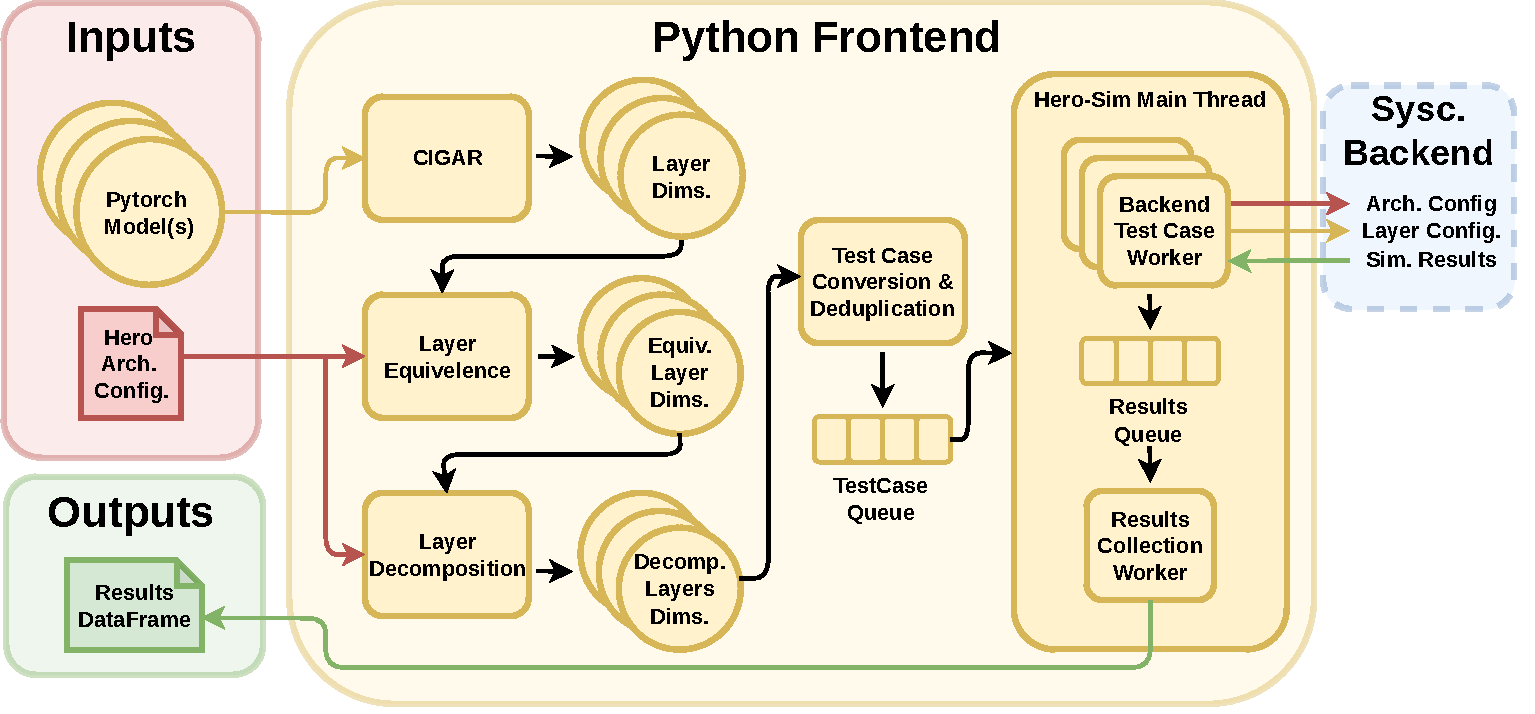
\includegraphics[scale=0.58]{fig/hero-sim-frontend.pdf}
    \caption{Illustration of the simulation enviornment's python frontend}
    \label{fig:frontend}
\end{figure}


\subsection{SystemC backend}
\label{chap:hero:sim_platform:backend}

The SystemC backend depicted in \autoref{fig:backend}, expects all inputs to be passed in as command line
arguments. The main inputs are the 1) architecture configuration and 2) layer
configuration needed for simulation by the frontend. Sim results are generated
and sent back to the frontend using protobufs. The backend first instantiates a
HERO instance using the architecute configuration passed as input. Then it
generates an equivelent layer based on the input layer configuration. Finally
using both layer and architecture configuration it generates the SAM descriptors
required to perform all data movement operations on-chip. A dram load is then
simulated in zero time to transfer the layer data and descriptors to the on-chip
memories of the newly constructed HERO instance. Once the initialized HERO
instance is ready, the cycle accurate simulation starts and continues until all
SAMs reach a suspend descriptor. Then a dram load operation is again performed
in zero time to transfer the results from the HERO instance for validation.
After the simulated dram load, a protobuf is constructed, then populated with
the result of ouput validation and simulation results (assuming validation
success) and sent back to the frontend for further analysis and aggregation. 

The backend simulates interactions between the architecture and DRAM
functionally, in zero-time to avoid the complexity of DRAM and SAM interactions.
The interaction between SAMs and DRAM are left as part of future work. 

\begin{figure}[ht]
    \centering
    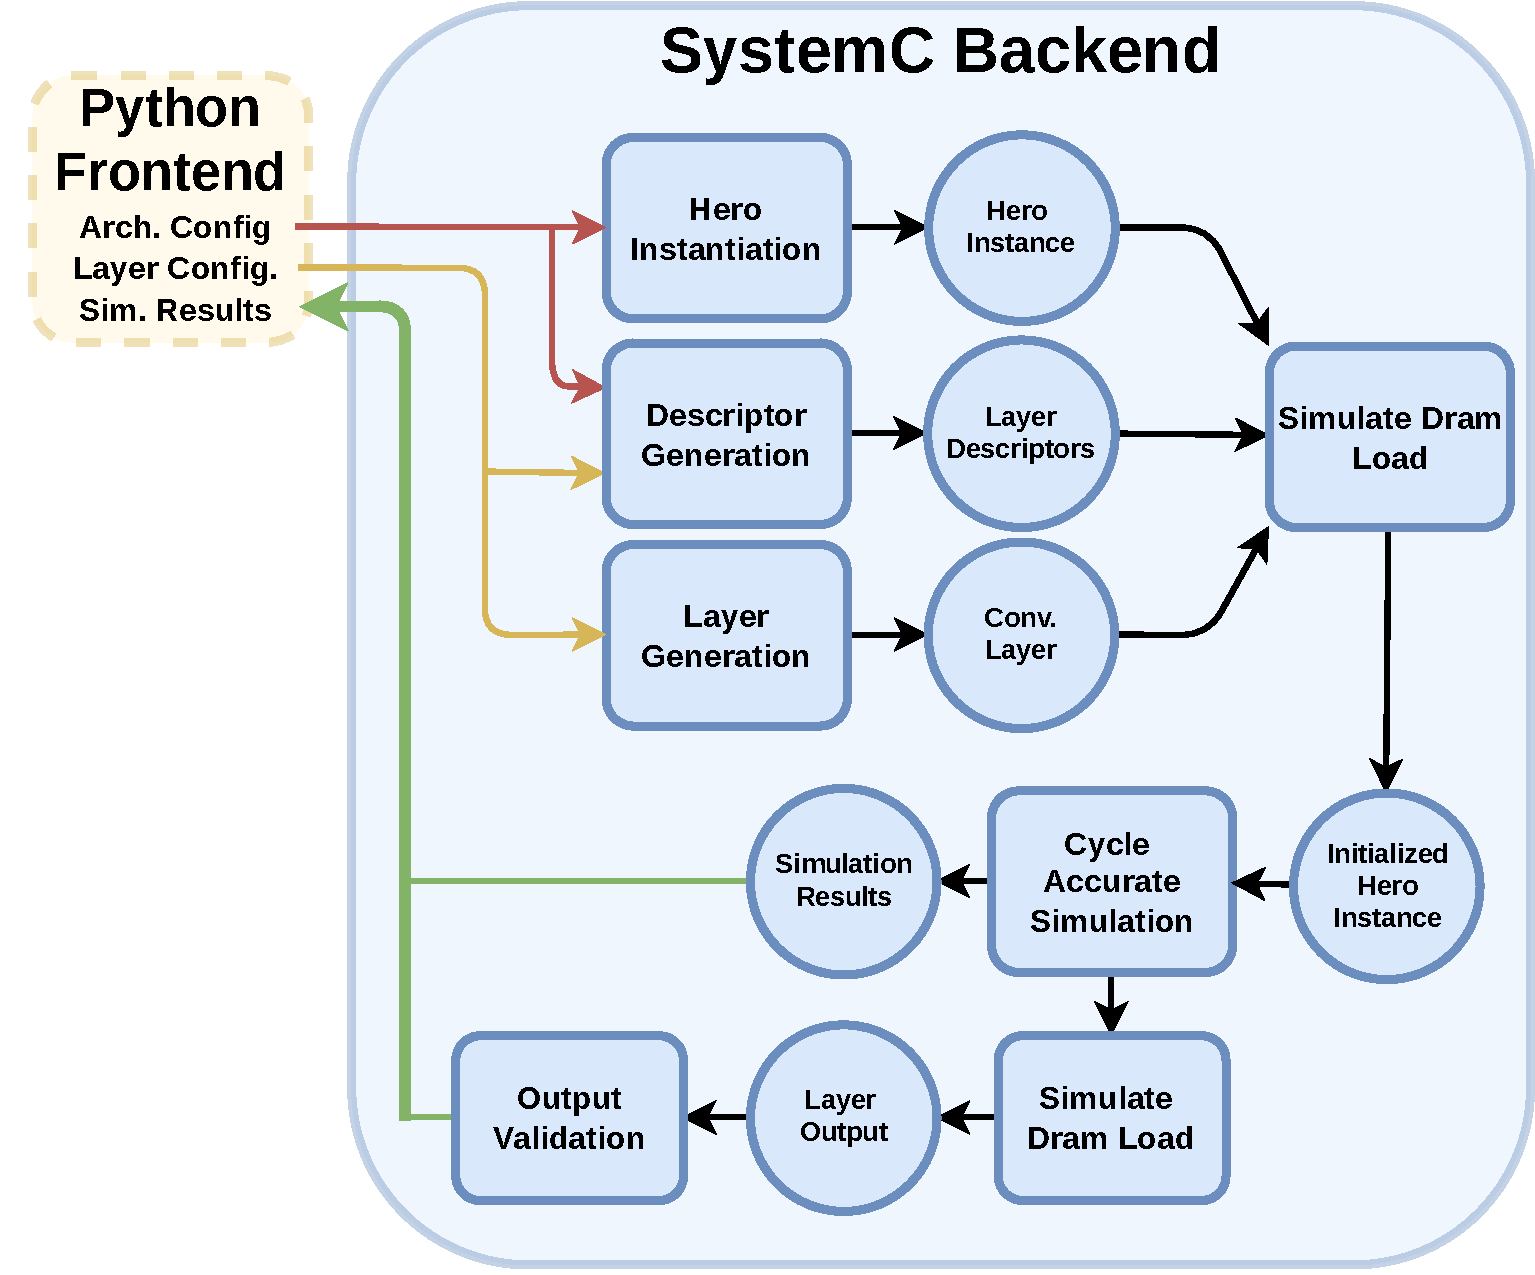
\includegraphics[scale=0.5]{fig/hero-sim-backend.pdf}
    \caption{Illustration of the simulation enviornment's SystemC backend}
    \label{fig:backend}
\end{figure}

\section{Experimental Results}
\label{chap:hero:results}

The configuration for the simulated architecture is given in
\autoref{tab:hero_config} based on the dimensions discovered in
\autoref{chap:dataflow_dse:exploring:results} and the sizing conclusions from
\autoref{chap:dataflow_dse:memory_hierarchy_sizing}. The CPU baseline used in
this work is an AMD 5950X processor. 

\begin{table}[]
    \center
    \begin{tabular}{|l|l|}
    \toprule
    Config. Param. & On-Chip Storage in Bytes    \\ 
    \midrule
    Weight Storage            & 16 B / PE (8 bit precision)  \\ \hline
    IFmap L3 Storage          & 1 MB (8 bit precision)   \\ \hline
    IFmap L2 Storage          & 512 B (8 bit precision)   \\ \hline
    OFmap Storage             & 1 MB (16 bit precision)   \\ \hline
    $C_{unroll}$              & 18   \\ \hline
    $f_{unroll}$              & 32   \\ \hline
    Directly Supported Kernels             & {(1, 1), (3, 3)}   \\ \hline
    Assumed CLK Speed             & 1 Ghz   \\ \hline
\end{tabular}
\caption{HERO configuration used for analysis}
\label{tab:hero_config}
\end{table}

\subsection{Percent of network compute for supported layers}
\label{chap:hero:sim_platform:cigar_side}

layers supported represent a substantial amount of total compute by network
how do I compute that since ops may be hard to estimate for some layers?
using runtime

\begin{figure}[ht]
    \centering
    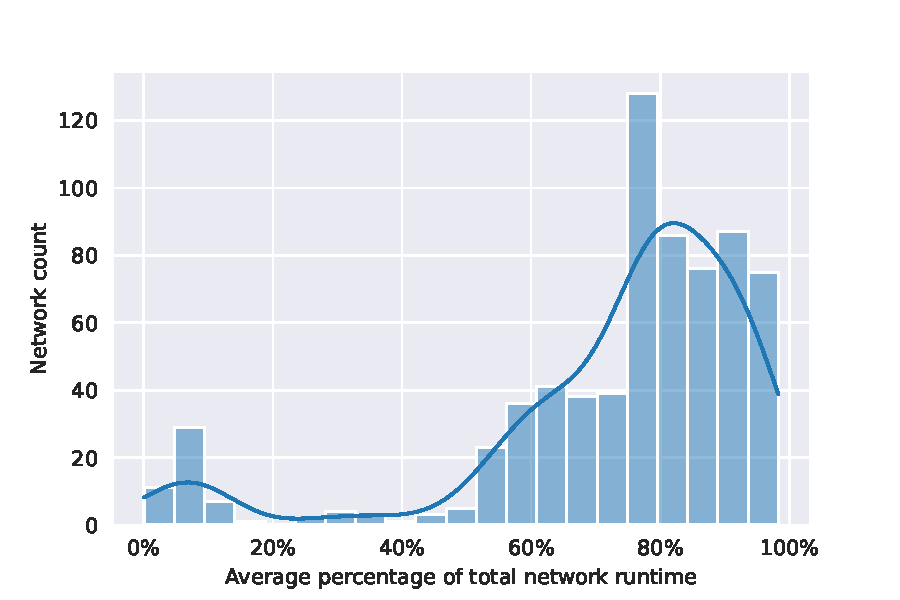
\includegraphics[scale=0.58]{Plots/overview/percent.pdf}
    \caption{Hardware Implementation Taxonomy adapted from \cite{maestro}}
    \label{fig:hw_taxonomy}
\end{figure}

\subsection{Utilization}
\label{chap:hero:sim_platform:cigar_side}

utilization is a surrogate for how well layers map to the architecture
some networks benefit substantially from the architecture
others don't. 

network level distribution of utilization is generally flat with
about a third not benefiting enough from the architecture due to low
utilization. 


\begin{figure}[ht]
    \centering
    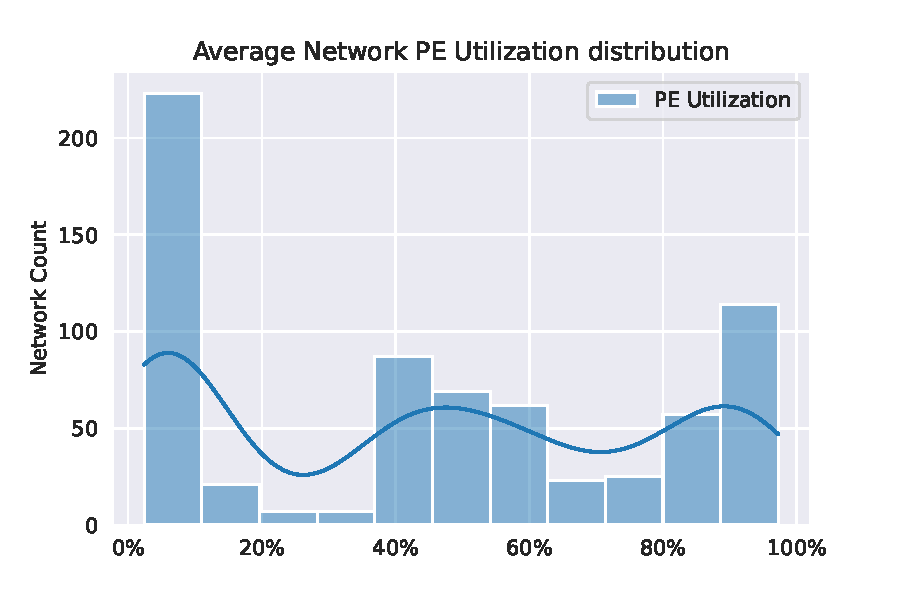
\includegraphics[scale=0.58]{Plots/utilization/network.pdf}
    \caption{Hardware Implementation Taxonomy adapted from \cite{maestro}}
    \label{fig:hw_taxonomy}
\end{figure}


At a more granular level it seems like utilization is bimodal

\begin{figure}[ht]
    \centering
    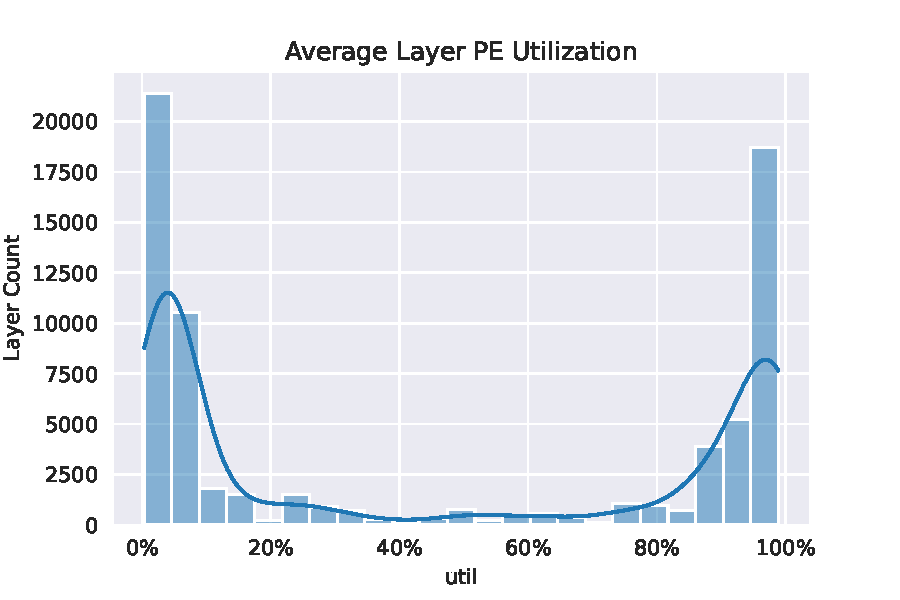
\includegraphics[scale=0.58]{Plots/utilization/layers.pdf}
    \caption{Hardware Implementation Taxonomy adapted from \cite{maestro}}
    \label{fig:hw_taxonomy}
\end{figure}

if utilization is low for small layers that would make sense
plotting utilization vs macs we see that we see that generally there's a trend where low
utilization correlates with lower macs
but there is a bulge MACS where high Macs correlates
with low utilization. Why? 

\begin{figure}[ht]
    \centering
    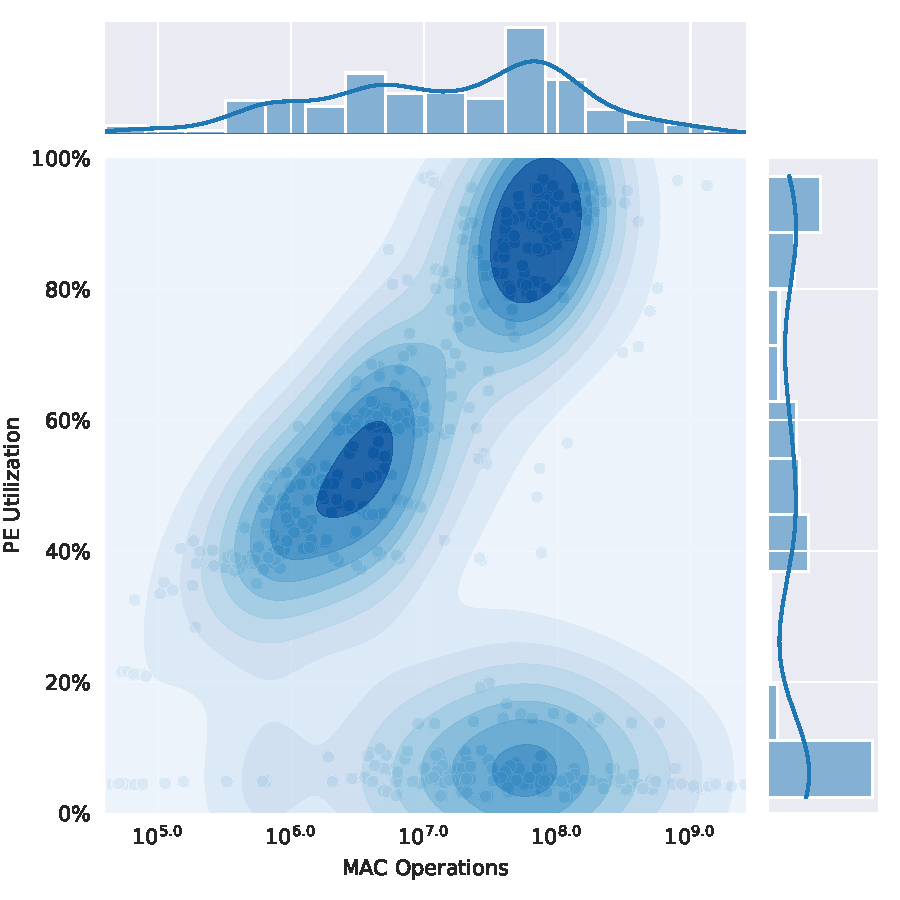
\includegraphics[scale=0.58]{Plots/utilization/util_vs_macs.pdf}
    \caption{Hardware Implementation Taxonomy adapted from \cite{maestro}}
    \label{fig:hw_taxonomy}
\end{figure}


Maybe layer decomposition and on chip memory plays a role here
Scatter plot of layers with speedup < 1 

\begin{figure}[ht]
    \centering
    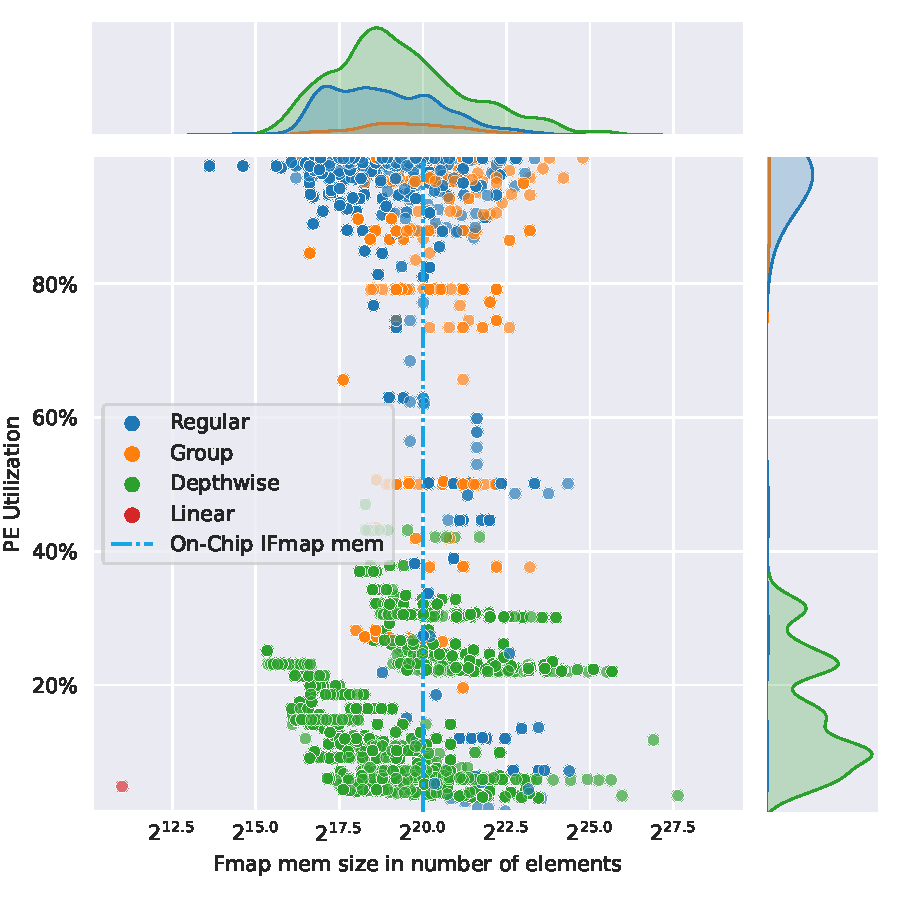
\includegraphics[scale=0.58]{Plots/utilization/util_vs_fmap.pdf}
    \caption{Hardware Implementation Taxonomy adapted from \cite{maestro}}
    \label{fig:hw_taxonomy}
\end{figure}


Misteriously theres  a cluster of layers with high utilization and low speedup
they fall on bouth sides of the on-chip memory line

If we look at types of layers that have low util and low speedup they're all
depthwise layers which are decomposed by group and poorly map to the
architecture

\begin{figure}[ht]
    \centering
    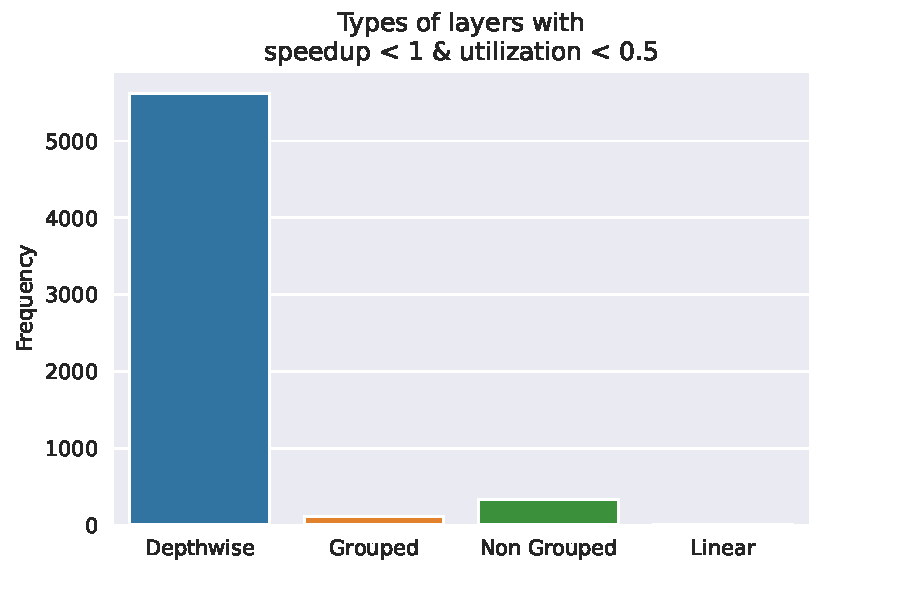
\includegraphics[scale=0.58]{Plots/utilization/type_of_low_util.pdf}
    \caption{Hardware Implementation Taxonomy adapted from \cite{maestro}}
    \label{fig:hw_taxonomy}
\end{figure}


If we look at layers with large footprint and low speedup they're size limits
concurrency because the full throughput of on-chip memory can't be used, these
layers need us to exploit a different kind of concurrency other than F, C Ky and
KX

\begin{figure}[ht]
    \centering
    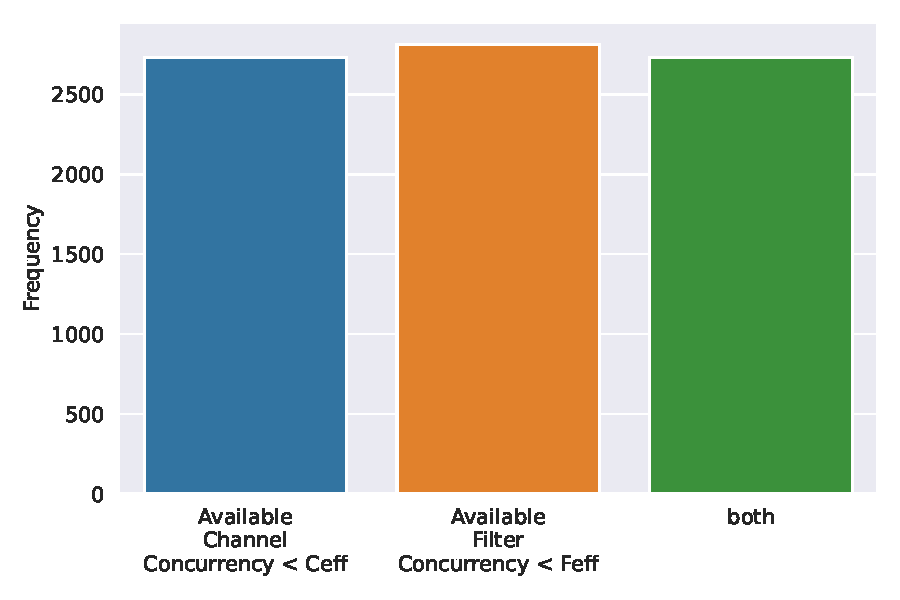
\includegraphics[scale=0.58]{Plots/utilization/low_util_big_fmap.pdf}
    % \caption{Rzeason for low utilization in layers with:\n speedup < 1\n" + "utilization < " + str(util_ub) +'\n' + r"memory footprint > $2^{20}$ elements}
    \label{fig:hw_taxonomy}
\end{figure}

what about layers with high utilization but low speedup
Not enough PES because of some many channels and filters

\begin{figure}[ht]
    \centering
    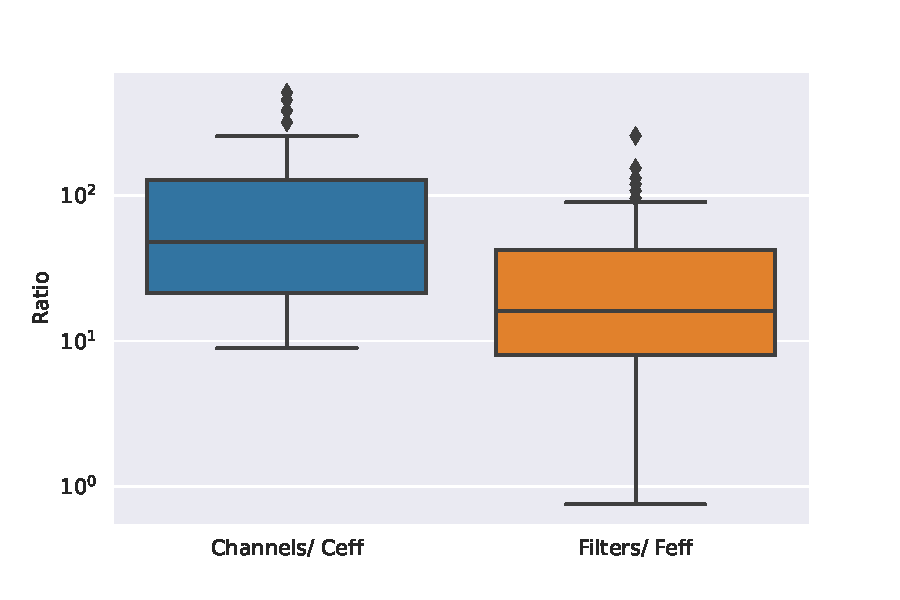
\includegraphics[scale=0.58]{Plots/utilization/ratios.pdf}
    \caption{Hardware Implementation Taxonomy adapted from \cite{maestro}}
    \label{fig:hw_taxonomy}
\end{figure}

Why the increase?
Lowering causes increase in layer macs
\begin{figure}[ht]
    \centering
    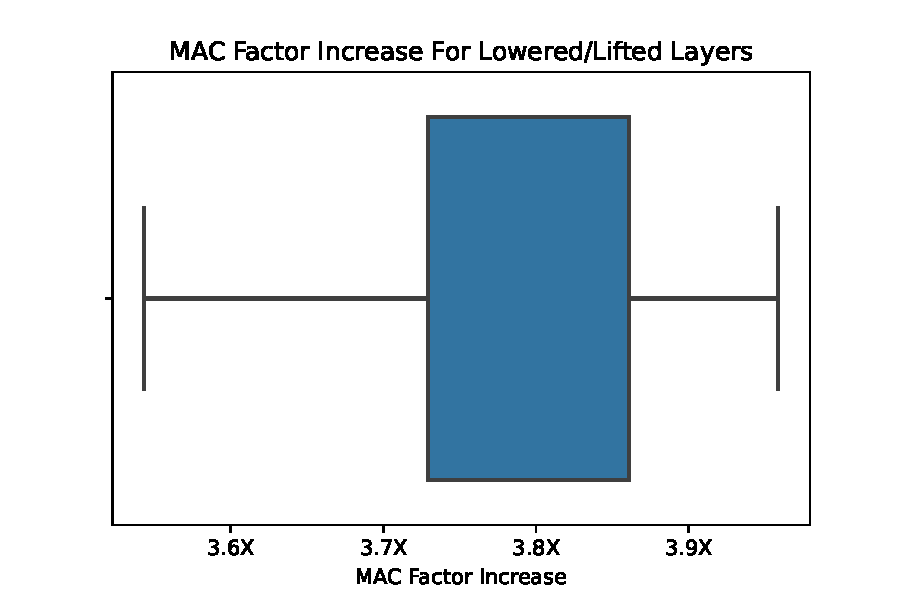
\includegraphics[scale=0.58]{Plots/utilization/macs.pdf}
    \caption{Hardware Implementation Taxonomy adapted from \cite{maestro}}
    \label{fig:hw_taxonomy}
\end{figure}

summary barplot

\begin{figure}[ht]
    \centering
    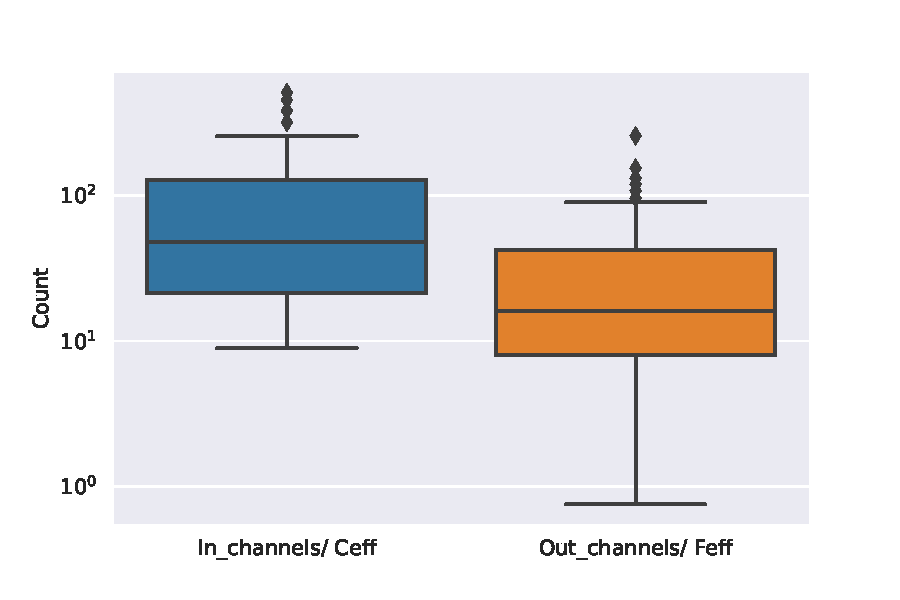
\includegraphics[scale=0.58]{Plots/utilization/summary.pdf}
    \caption{Hardware Implementation Taxonomy adapted from \cite{maestro}}
    \label{fig:hw_taxonomy}
\end{figure}

\subsection{Latency and Speedup over CPU Baseline}
\label{chap:hero:sim_platform:cigar_side}

most networks/ layers benefit
median network speedup over 

\begin{figure}[ht]
    \centering
    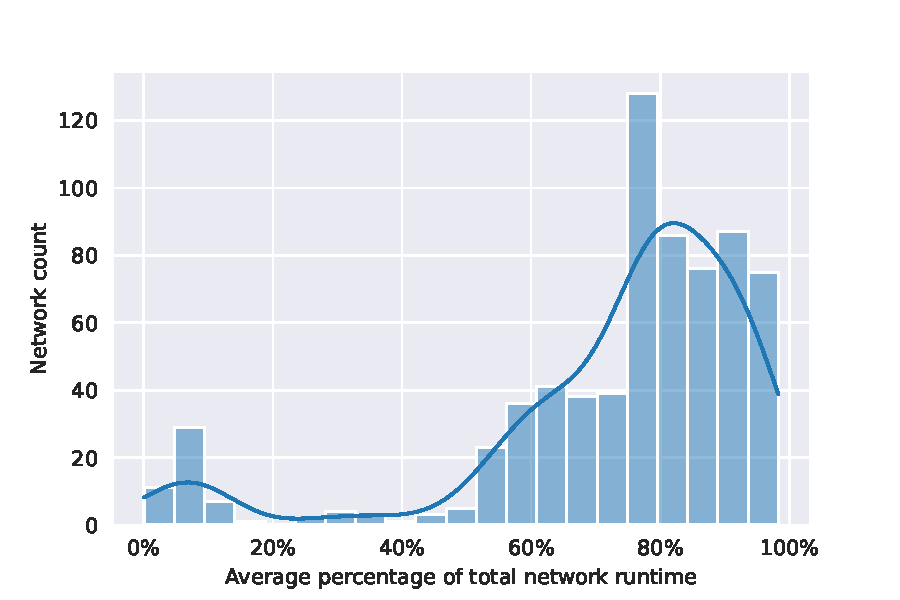
\includegraphics[scale=0.58]{Plots/overview/percent.pdf}
    \caption{Hardware Implementation Taxonomy adapted from \cite{maestro}}
    \label{fig:hw_taxonomy}
\end{figure}

Some networks don't benefit

\begin{figure}[ht]
    \centering
    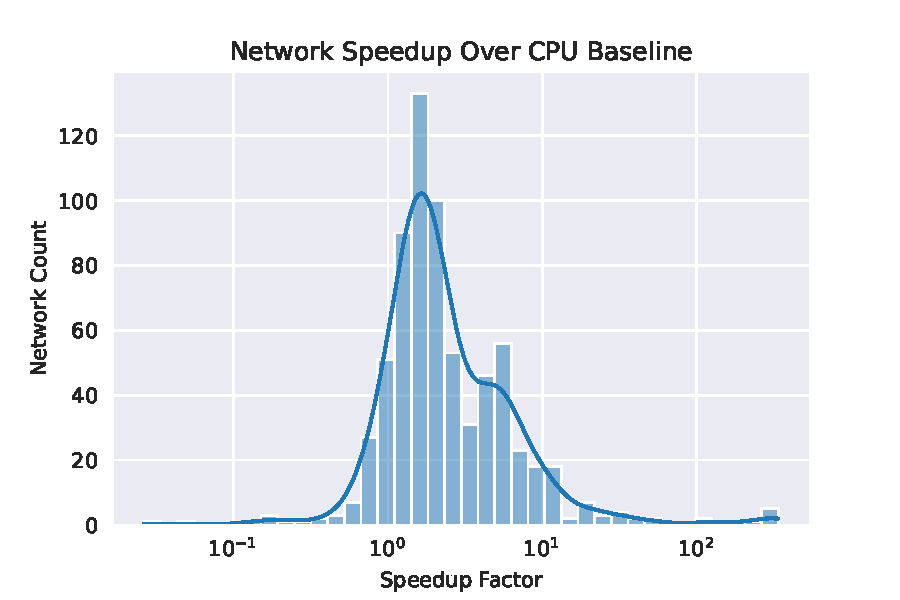
\includegraphics[scale=0.58]{Plots/latency/net_speedup.pdf}
    \caption{Hardware Implementation Taxonomy adapted from \cite{maestro}}
    \label{fig:hw_taxonomy}
\end{figure}

12\% of layers don't benefit

\begin{figure}[ht]
    \centering
    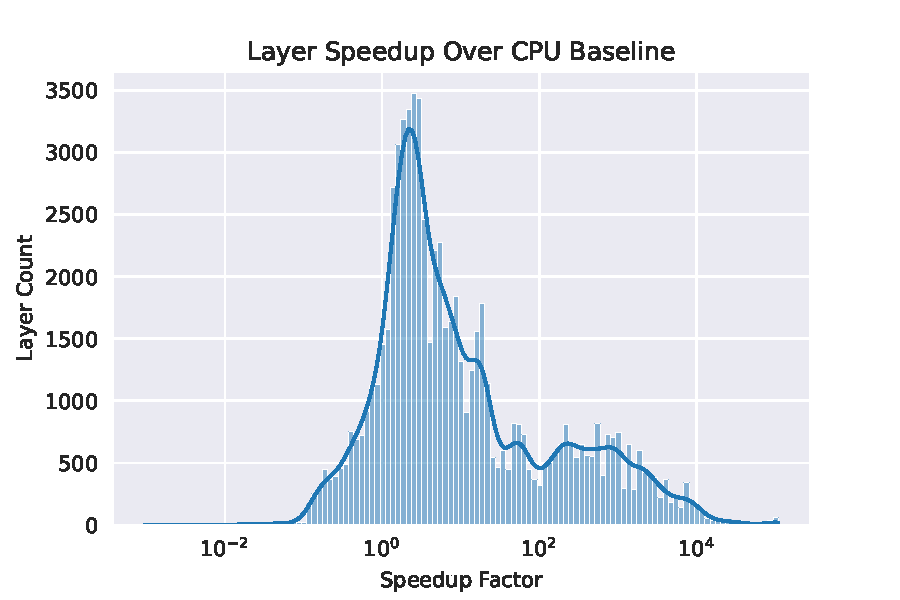
\includegraphics[scale=0.58]{Plots/latency/layer_speedup.pdf}
    \caption{Hardware Implementation Taxonomy adapted from \cite{maestro}}
    \label{fig:hw_taxonomy}
\end{figure}


why? see utilization
here's a boxplot of per layer speedup excluding layers with no speedup

\begin{figure}[ht]
    \centering
    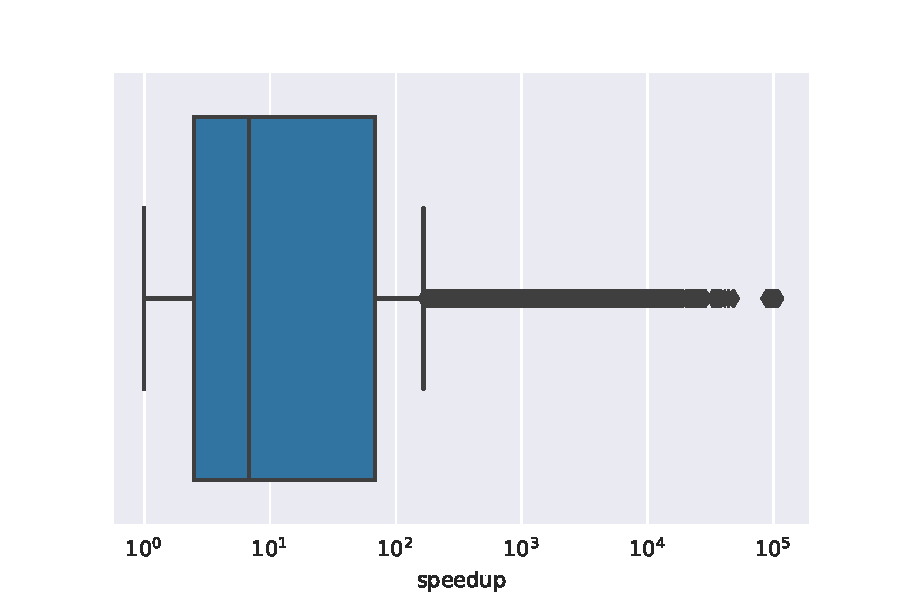
\includegraphics[scale=0.58]{Plots/latency/speedup_gt_1_boxplot.pdf}
    \caption{Hardware Implementation Taxonomy adapted from \cite{maestro}}
    \label{fig:hw_taxonomy}
\end{figure}

estimated fps based on supported layers, note that this should be taken as upper
bound because unsupported supported layers may take up more of the runtime than
anticipated (references earlier figure)

\begin{figure}[ht]
    \centering
    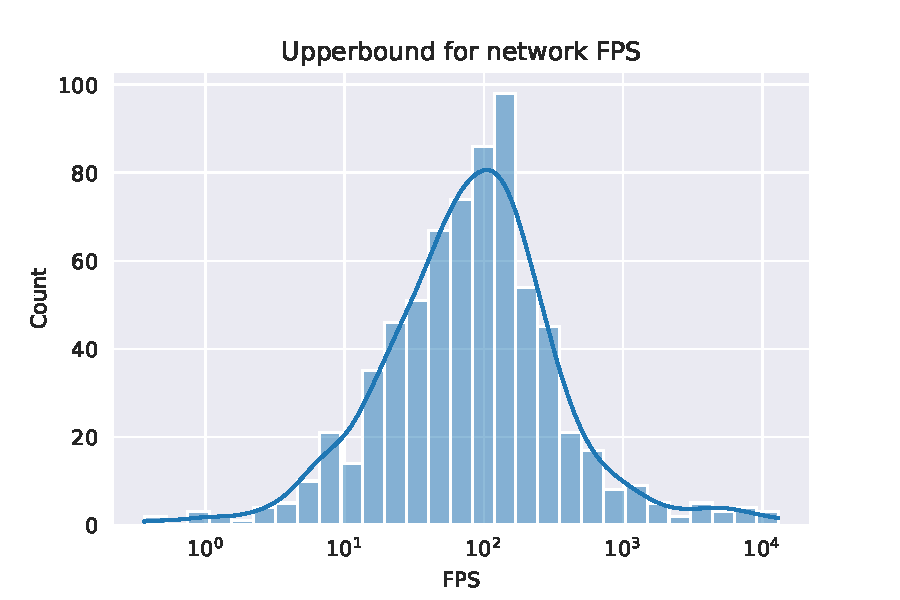
\includegraphics[scale=0.58]{Plots/latency/fps.pdf}
    \caption{Hardware Implementation Taxonomy adapted from \cite{maestro}}
    \label{fig:hw_taxonomy}
\end{figure}



\subsection{DRAM Bandwidth}
\label{chap:hero:sim_platform:cigar_side}

network and layer bandwidth histograms
within ddr4 spec

\begin{figure}[ht]
    \centering
    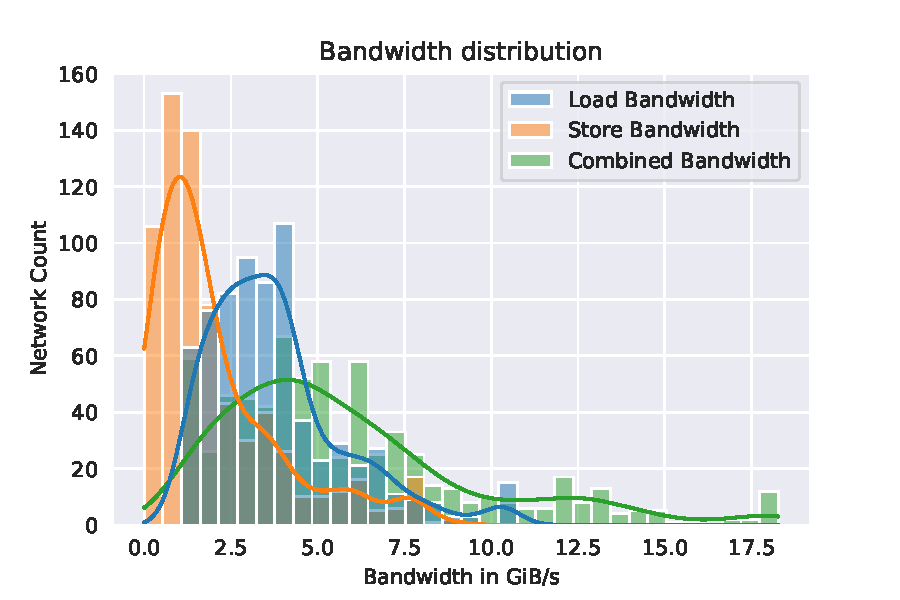
\includegraphics[scale=0.58]{Plots/resources/net_bw.pdf}
    \caption{Hardware Implementation Taxonomy adapted from \cite{maestro}}
    \label{fig:hw_taxonomy}
\end{figure}


\subsection{Energy}
\label{chap:hero:sim_platform:cigar_side}

used energy model in cite energy model
add energy model as table

\begin{figure}[ht]
    \centering
    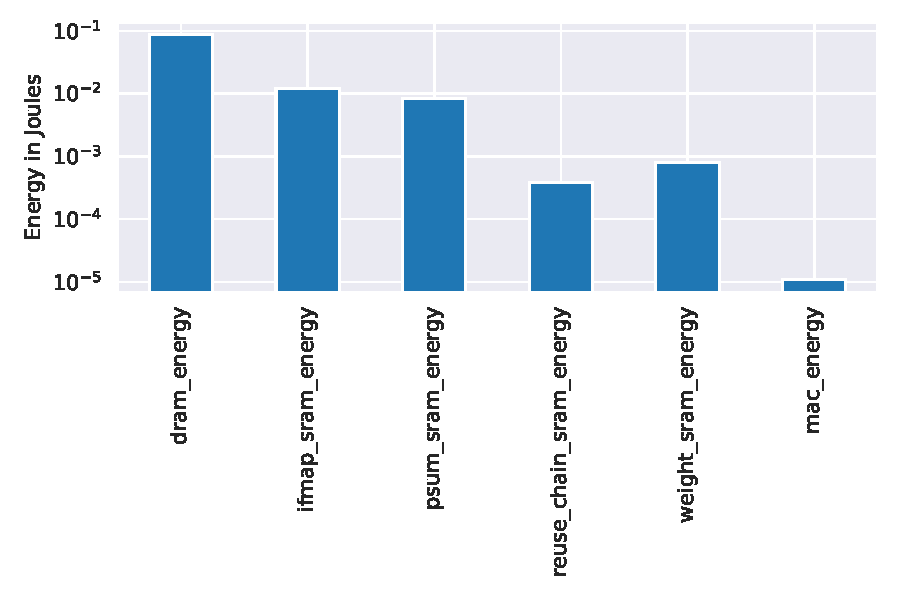
\includegraphics[scale=0.58]{Plots/energy/barplot.pdf}
    \caption{Hardware Implementation Taxonomy adapted from \cite{maestro}}
    \label{fig:hw_taxonomy}
\end{figure}

mac is basically free
dram dominates


network inferences/ j median is around 57

\begin{figure}[ht]
    \centering
    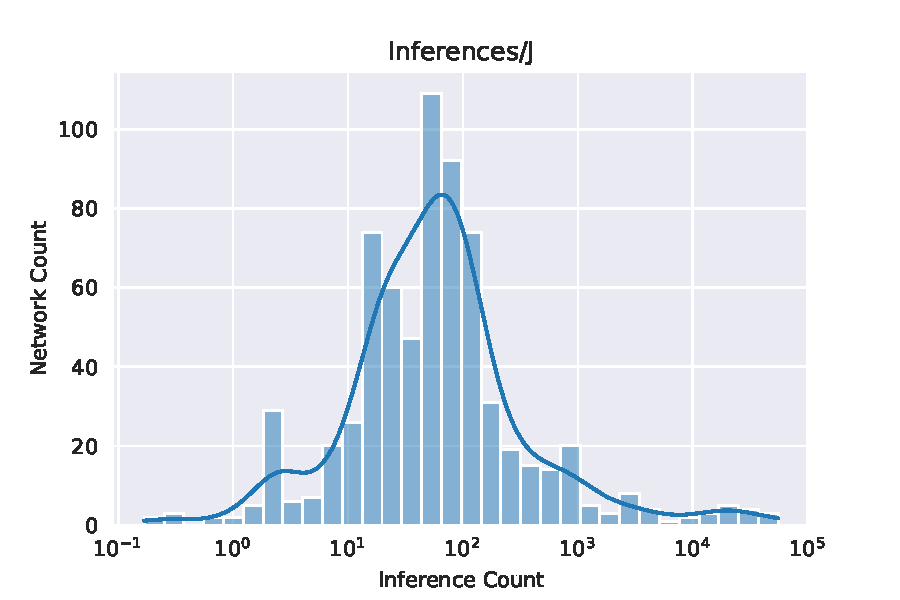
\includegraphics[scale=0.58]{Plots/energy/inferences.pdf}
    \caption{Hardware Implementation Taxonomy adapted from \cite{maestro}}
    \label{fig:hw_taxonomy}
\end{figure}


excluding dram number jumps to 20K
there's room to reduce on-chip data movement by exploiting different kinds of
concurrency

\begin{figure}[ht]
    \centering
    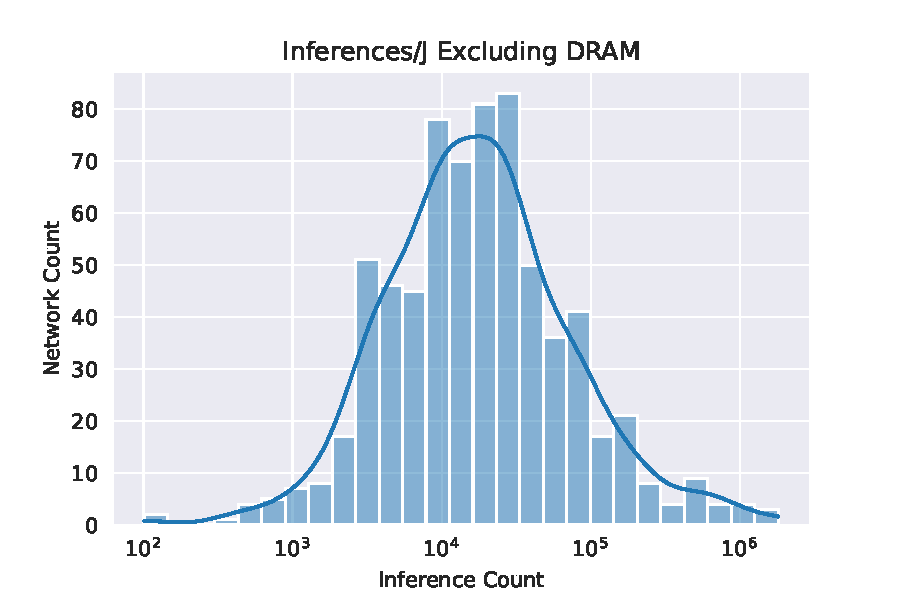
\includegraphics[scale=0.58]{Plots/energy/inferences_wo_dram.pdf}
    \caption{Hardware Implementation Taxonomy adapted from \cite{maestro}}
    \label{fig:hw_taxonomy}
\end{figure}

\subsection{Area}
\label{chap:conv_gemm_equiv:overhead}

area model as table
bulk goes to ofmap storage and ifmap storage
ofmap storage requires higher precision

\begin{figure}[ht]
    \centering
    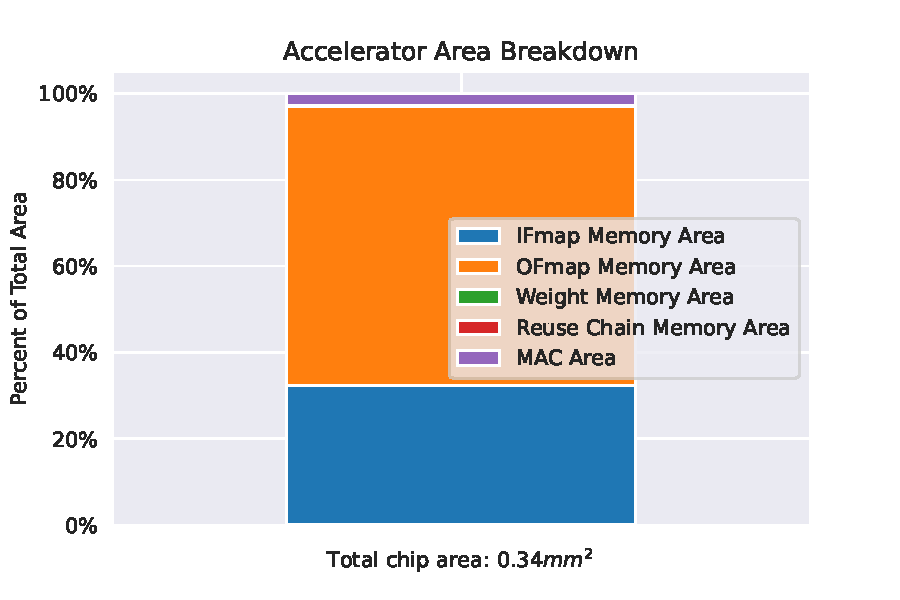
\includegraphics[scale=0.58]{Plots/resources/area.pdf}
    \caption{Hardware Implementation Taxonomy adapted from \cite{maestro}}
    \label{fig:hw_taxonomy}
\end{figure}

\subsection{Descriptor program scaling}
\label{chap:hero:sim_platform:cigar_side}

median required storage for descriptors per address generator is around 100
scaling can be improved with more complicated descriptors

\begin{figure}[ht]
    \centering
    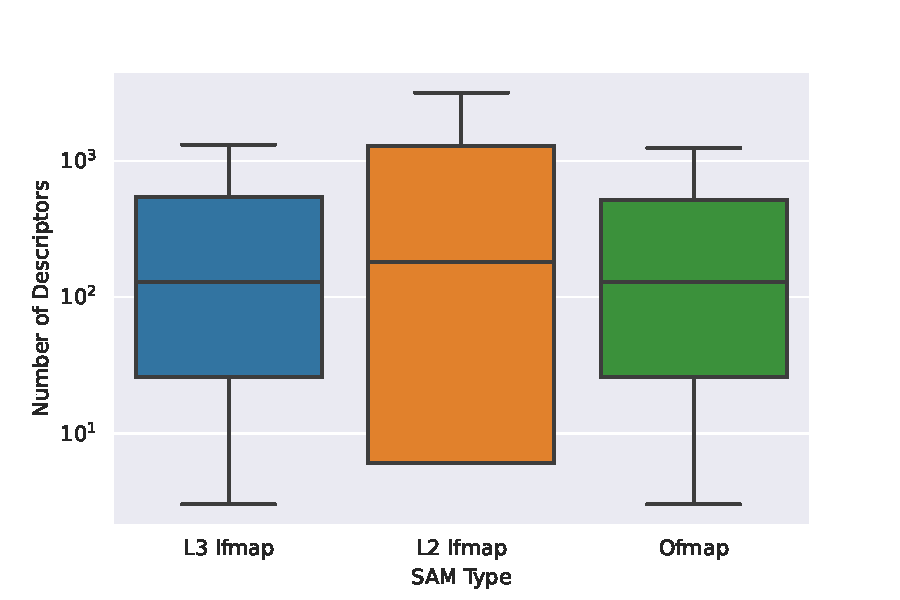
\includegraphics[scale=0.58]{Plots/resources/descriptors.pdf}
    \caption{Hardware Implementation Taxonomy adapted from \cite{maestro}}
    \label{fig:hw_taxonomy}
\end{figure}

\subsection{Per network results}
\label{chap:hero:sim_platform:cigar_side}

networks chosen
resnet50 (popular and backbone for alot of other networks)
mobilenetv3 specific to edge devices and has depthwise layers (let's see effect
of offloading on cpu)
hrnet18 flexible network used for variety of tasks, also has larger layers

\subsubsection{ResNet50}

\clearpage
\begin{center}
    \begin{tabular}{lrlrrlllll}
        \toprule
        {} &  Count & IFmap &     Cin &    Cout &       K &  Stride & Padding & Groups &   Bias \\
        Name     &        &             &         &         &         &         &         &        &        \\
        \midrule
        conv\_0   & 1 &  (224, 224) &     3.0 &    64.0 &  (7, 7) &  (2, 2) &  (3, 3) &    1.0 &  False \\
        conv\_1   & 1 &    (56, 56) &    64.0 &    64.0 &  (1, 1) &  (1, 1) &  (0, 0) &    1.0 &  False \\
        conv\_2   & 3 &    (56, 56) &    64.0 &    64.0 &  (3, 3) &  (1, 1) &  (1, 1) &    1.0 &  False \\
        conv\_3   & 4 &    (56, 56) &    64.0 &   256.0 &  (1, 1) &  (1, 1) &  (0, 0) &    1.0 &  False \\
        conv\_4   & 2 &    (56, 56) &   256.0 &    64.0 &  (1, 1) &  (1, 1) &  (0, 0) &    1.0 &  False \\
        conv\_5   & 1 &    (56, 56) &   256.0 &   128.0 &  (1, 1) &  (1, 1) &  (0, 0) &    1.0 &  False \\
        conv\_6   & 1 &    (56, 56) &   128.0 &   128.0 &  (3, 3) &  (2, 2) &  (1, 1) &    1.0 &  False \\
        conv\_7   & 4 &    (28, 28) &   128.0 &   512.0 &  (1, 1) &  (1, 1) &  (0, 0) &    1.0 &  False \\
        conv\_8   & 1 &    (56, 56) &   256.0 &   512.0 &  (1, 1) &  (2, 2) &  (0, 0) &    1.0 &  False \\
        conv\_9   & 3 &    (28, 28) &   512.0 &   128.0 &  (1, 1) &  (1, 1) &  (0, 0) &    1.0 &  False \\
        conv\_10  & 3 &    (28, 28) &   128.0 &   128.0 &  (3, 3) &  (1, 1) &  (1, 1) &    1.0 &  False \\
        conv\_11  & 1 &    (28, 28) &   512.0 &   256.0 &  (1, 1) &  (1, 1) &  (0, 0) &    1.0 &  False \\
        conv\_12  & 1 &    (28, 28) &   256.0 &   256.0 &  (3, 3) &  (2, 2) &  (1, 1) &    1.0 &  False \\
        conv\_13  & 6 &    (14, 14) &   256.0 &  1024.0 &  (1, 1) &  (1, 1) &  (0, 0) &    1.0 &  False \\
        conv\_14  & 1 &    (28, 28) &   512.0 &  1024.0 &  (1, 1) &  (2, 2) &  (0, 0) &    1.0 &  False \\
        conv\_15  & 5 &    (14, 14) &  1024.0 &   256.0 &  (1, 1) &  (1, 1) &  (0, 0) &    1.0 &  False \\
        conv\_16  & 5 &    (14, 14) &   256.0 &   256.0 &  (3, 3) &  (1, 1) &  (1, 1) &    1.0 &  False \\
        conv\_17  & 1 &    (14, 14) &  1024.0 &   512.0 &  (1, 1) &  (1, 1) &  (0, 0) &    1.0 &  False \\
        conv\_18  & 1 &    (14, 14) &   512.0 &   512.0 &  (3, 3) &  (2, 2) &  (1, 1) &    1.0 &  False \\
        conv\_19  & 3 &      (7, 7) &   512.0 &  2048.0 &  (1, 1) &  (1, 1) &  (0, 0) &    1.0 &  False \\
        conv\_20  & 1 &    (14, 14) &  1024.0 &  2048.0 &  (1, 1) &  (2, 2) &  (0, 0) &    1.0 &  False \\
        conv\_21  & 2 &      (7, 7) &  2048.0 &   512.0 &  (1, 1) &  (1, 1) &  (0, 0) &    1.0 &  False \\
        conv\_22  & 2 &      (7, 7) &   512.0 &   512.0 &  (3, 3) &  (1, 1) &  (1, 1) &    1.0 &  False \\
        linear\_0 & 1 &      (1, 1) &  2048.0 &  1000.0 &     N/A &     N/A &     N/A &    N/A &   True \\
        \bottomrule
        \end{tabular}
\end{center}

\begin{figure}[ht]
    \centering
    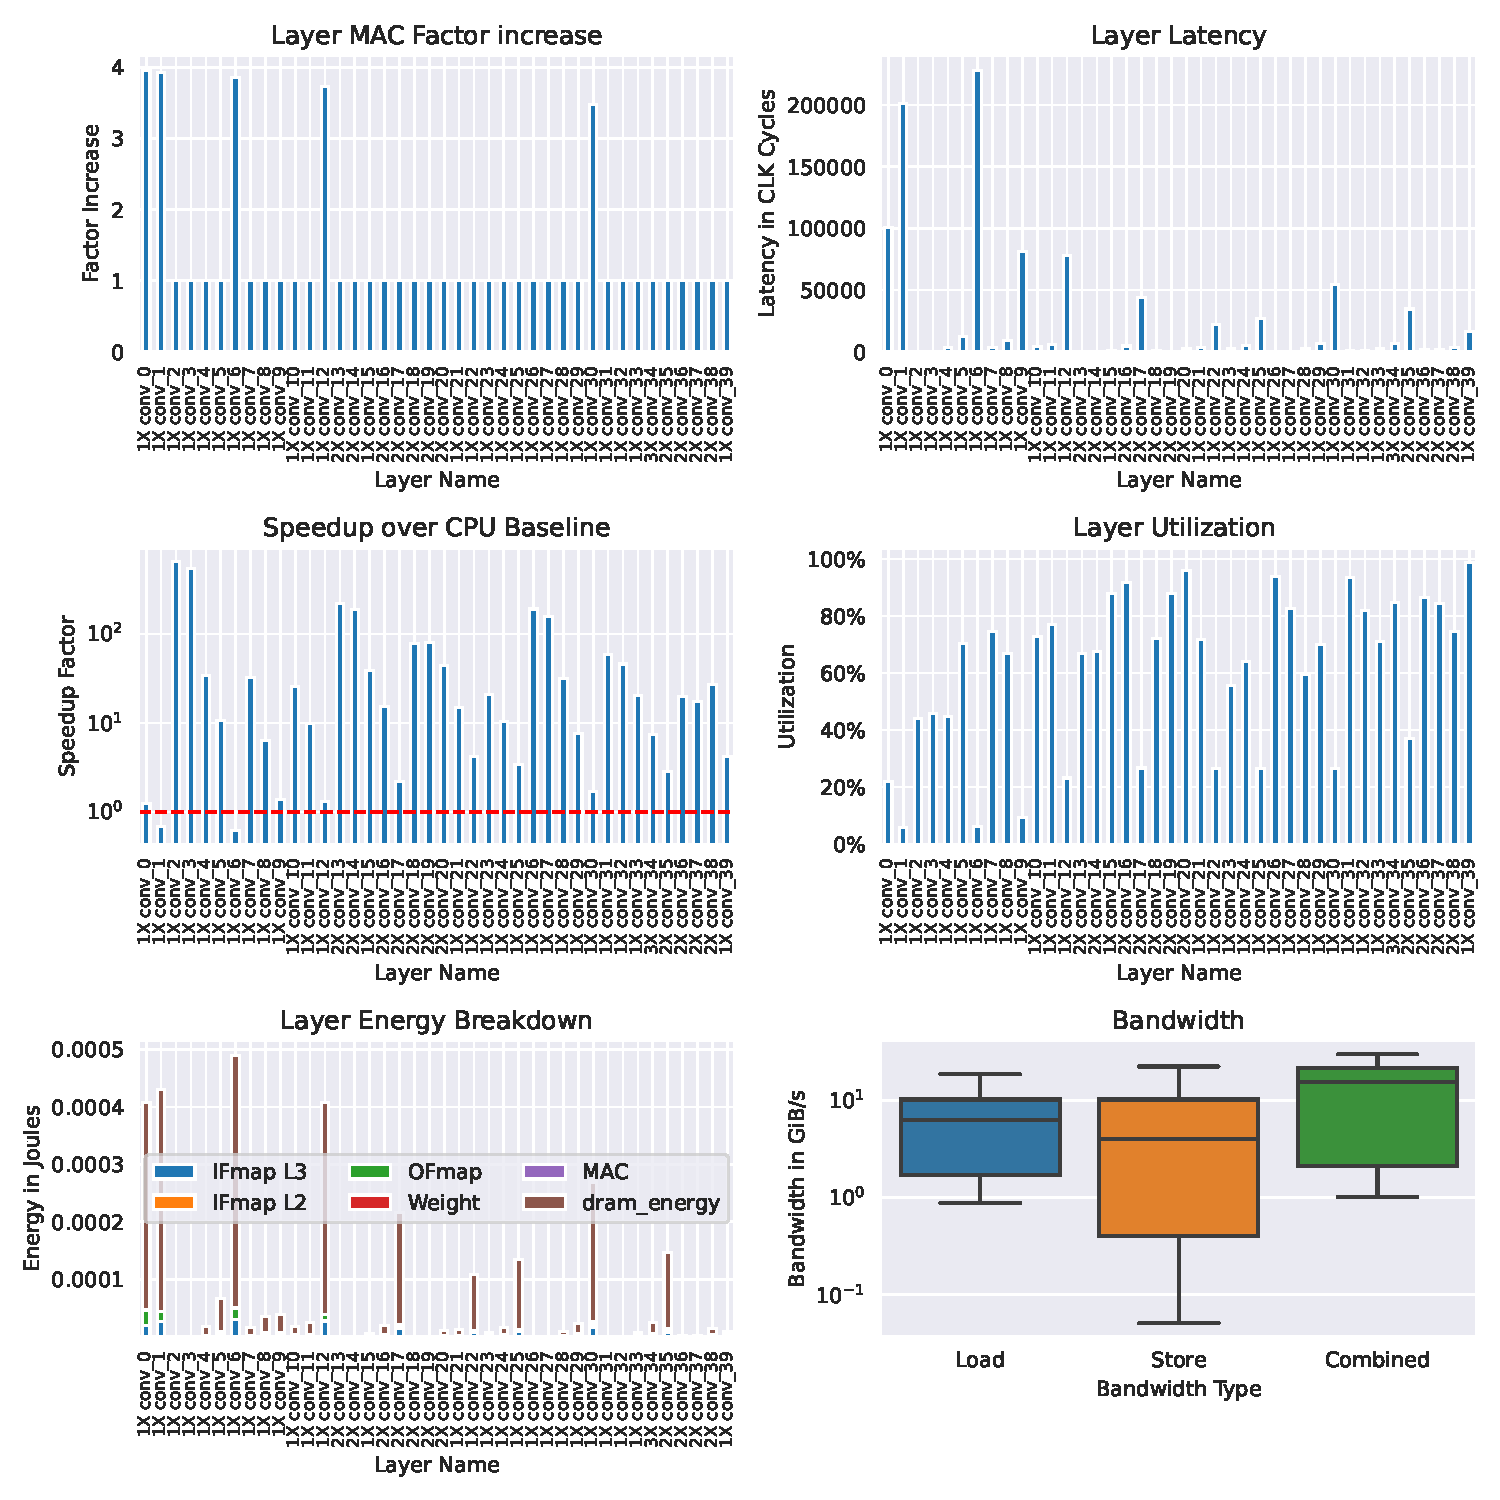
\includegraphics[scale=0.6]{Plots/networks/mobilenetv3_small_075.pdf}
    \caption{Hardware Implementation Taxonomy adapted from \cite{maestro}}
    \label{fig:hw_taxonomy}
\end{figure}

\subsubsection{MobilenetV3}

\clearpage
% \Rotatebox{90}{%
\begin{center}
    \begin{tabular}{lrlrrlllll}
        \toprule
        {} &  Count &       IFmap &    Cin &    Cout &       K &  Stride & Padding & Groups &   Bias \\
        Name    &        &             &        &         &         &         &         &        &        \\
        \midrule
        conv\_0  &      1 &  (224, 224) &    3.0 &    16.0 &  (3, 3) &  (2, 2) &  (1, 1) &    1.0 &  False \\
        conv\_1  &      1 &  (112, 112) &   16.0 &    16.0 &  (3, 3) &  (2, 2) &  (1, 1) &   16.0 &  False \\
        conv\_2  &      1 &      (1, 1) &   16.0 &     8.0 &  (1, 1) &  (1, 1) &  (0, 0) &    1.0 &   True \\
        conv\_3  &      1 &      (1, 1) &    8.0 &    16.0 &  (1, 1) &  (1, 1) &  (0, 0) &    1.0 &   True \\
        conv\_4  &      1 &    (56, 56) &   16.0 &    16.0 &  (1, 1) &  (1, 1) &  (0, 0) &    1.0 &  False \\
        conv\_5  &      1 &    (56, 56) &   16.0 &    72.0 &  (1, 1) &  (1, 1) &  (0, 0) &    1.0 &  False \\
        conv\_6  &      1 &    (56, 56) &   72.0 &    72.0 &  (3, 3) &  (2, 2) &  (1, 1) &   72.0 &  False \\
        conv\_7  &      1 &    (28, 28) &   72.0 &    24.0 &  (1, 1) &  (1, 1) &  (0, 0) &    1.0 &  False \\
        conv\_8  &      1 &    (28, 28) &   24.0 &    88.0 &  (1, 1) &  (1, 1) &  (0, 0) &    1.0 &  False \\
        conv\_9  &      1 &    (28, 28) &   88.0 &    88.0 &  (3, 3) &  (1, 1) &  (1, 1) &   88.0 &  False \\
        conv\_10 &      1 &    (28, 28) &   88.0 &    24.0 &  (1, 1) &  (1, 1) &  (0, 0) &    1.0 &  False \\
        conv\_11 &      1 &    (28, 28) &   24.0 &    96.0 &  (1, 1) &  (1, 1) &  (0, 0) &    1.0 &  False \\
        conv\_12 &      1 &    (28, 28) &   96.0 &    96.0 &  (5, 5) &  (2, 2) &  (2, 2) &   96.0 &  False \\
        conv\_13 &      2 &      (1, 1) &   96.0 &    24.0 &  (1, 1) &  (1, 1) &  (0, 0) &    1.0 &   True \\
        conv\_14 &      2 &      (1, 1) &   24.0 &    96.0 &  (1, 1) &  (1, 1) &  (0, 0) &    1.0 &   True \\
        conv\_15 &      1 &    (14, 14) &   96.0 &    32.0 &  (1, 1) &  (1, 1) &  (0, 0) &    1.0 &  False \\
        conv\_16 &      2 &    (14, 14) &   32.0 &   192.0 &  (1, 1) &  (1, 1) &  (0, 0) &    1.0 &  False \\
        conv\_17 &      2 &    (14, 14) &  192.0 &   192.0 &  (5, 5) &  (1, 1) &  (2, 2) &  192.0 &  False \\
        conv\_18 &      2 &      (1, 1) &  192.0 &    48.0 &  (1, 1) &  (1, 1) &  (0, 0) &    1.0 &   True \\
        conv\_19 &      2 &      (1, 1) &   48.0 &   192.0 &  (1, 1) &  (1, 1) &  (0, 0) &    1.0 &   True \\
        conv\_20 &      2 &    (14, 14) &  192.0 &    32.0 &  (1, 1) &  (1, 1) &  (0, 0) &    1.0 &  False \\
        conv\_21 &      1 &    (14, 14) &   32.0 &    96.0 &  (1, 1) &  (1, 1) &  (0, 0) &    1.0 &  False \\
        conv\_22 &      1 &    (14, 14) &   96.0 &    96.0 &  (5, 5) &  (1, 1) &  (2, 2) &   96.0 &  False \\
        conv\_23 &      1 &    (14, 14) &   96.0 &    40.0 &  (1, 1) &  (1, 1) &  (0, 0) &    1.0 &  False \\
        conv\_24 &      1 &    (14, 14) &   40.0 &   120.0 &  (1, 1) &  (1, 1) &  (0, 0) &    1.0 &  False \\
        conv\_25 &      1 &    (14, 14) &  120.0 &   120.0 &  (5, 5) &  (1, 1) &  (2, 2) &  120.0 &  False \\
        conv\_26 &      1 &      (1, 1) &  120.0 &    32.0 &  (1, 1) &  (1, 1) &  (0, 0) &    1.0 &   True \\
        conv\_27 &      1 &      (1, 1) &   32.0 &   120.0 &  (1, 1) &  (1, 1) &  (0, 0) &    1.0 &   True \\
        conv\_28 &      1 &    (14, 14) &  120.0 &    40.0 &  (1, 1) &  (1, 1) &  (0, 0) &    1.0 &  False \\
        conv\_29 &      1 &    (14, 14) &   40.0 &   240.0 &  (1, 1) &  (1, 1) &  (0, 0) &    1.0 &  False \\
        conv\_30 &      1 &    (14, 14) &  240.0 &   240.0 &  (5, 5) &  (2, 2) &  (2, 2) &  240.0 &  False \\
        conv\_31 &      1 &      (1, 1) &  240.0 &    64.0 &  (1, 1) &  (1, 1) &  (0, 0) &    1.0 &   True \\
        conv\_32 &      1 &      (1, 1) &   64.0 &   240.0 &  (1, 1) &  (1, 1) &  (0, 0) &    1.0 &   True \\
        conv\_33 &      1 &      (7, 7) &  240.0 &    72.0 &  (1, 1) &  (1, 1) &  (0, 0) &    1.0 &  False \\
        conv\_34 &      3 &      (7, 7) &   72.0 &   432.0 &  (1, 1) &  (1, 1) &  (0, 0) &    1.0 &  False \\
        conv\_35 &      2 &      (7, 7) &  432.0 &   432.0 &  (5, 5) &  (1, 1) &  (2, 2) &  432.0 &  False \\
        conv\_36 &      2 &      (1, 1) &  432.0 &   112.0 &  (1, 1) &  (1, 1) &  (0, 0) &    1.0 &   True \\
        conv\_37 &      2 &      (1, 1) &  112.0 &   432.0 &  (1, 1) &  (1, 1) &  (0, 0) &    1.0 &   True \\
        conv\_38 &      2 &      (7, 7) &  432.0 &    72.0 &  (1, 1) &  (1, 1) &  (0, 0) &    1.0 &  False \\
        conv\_39 &      1 &      (1, 1) &  432.0 &  1024.0 &  (1, 1) &  (1, 1) &  (0, 0) &    1.0 &   True \\
        \bottomrule
        \end{tabular}
\end{center}

\begin{figure}[ht]
    \centering
    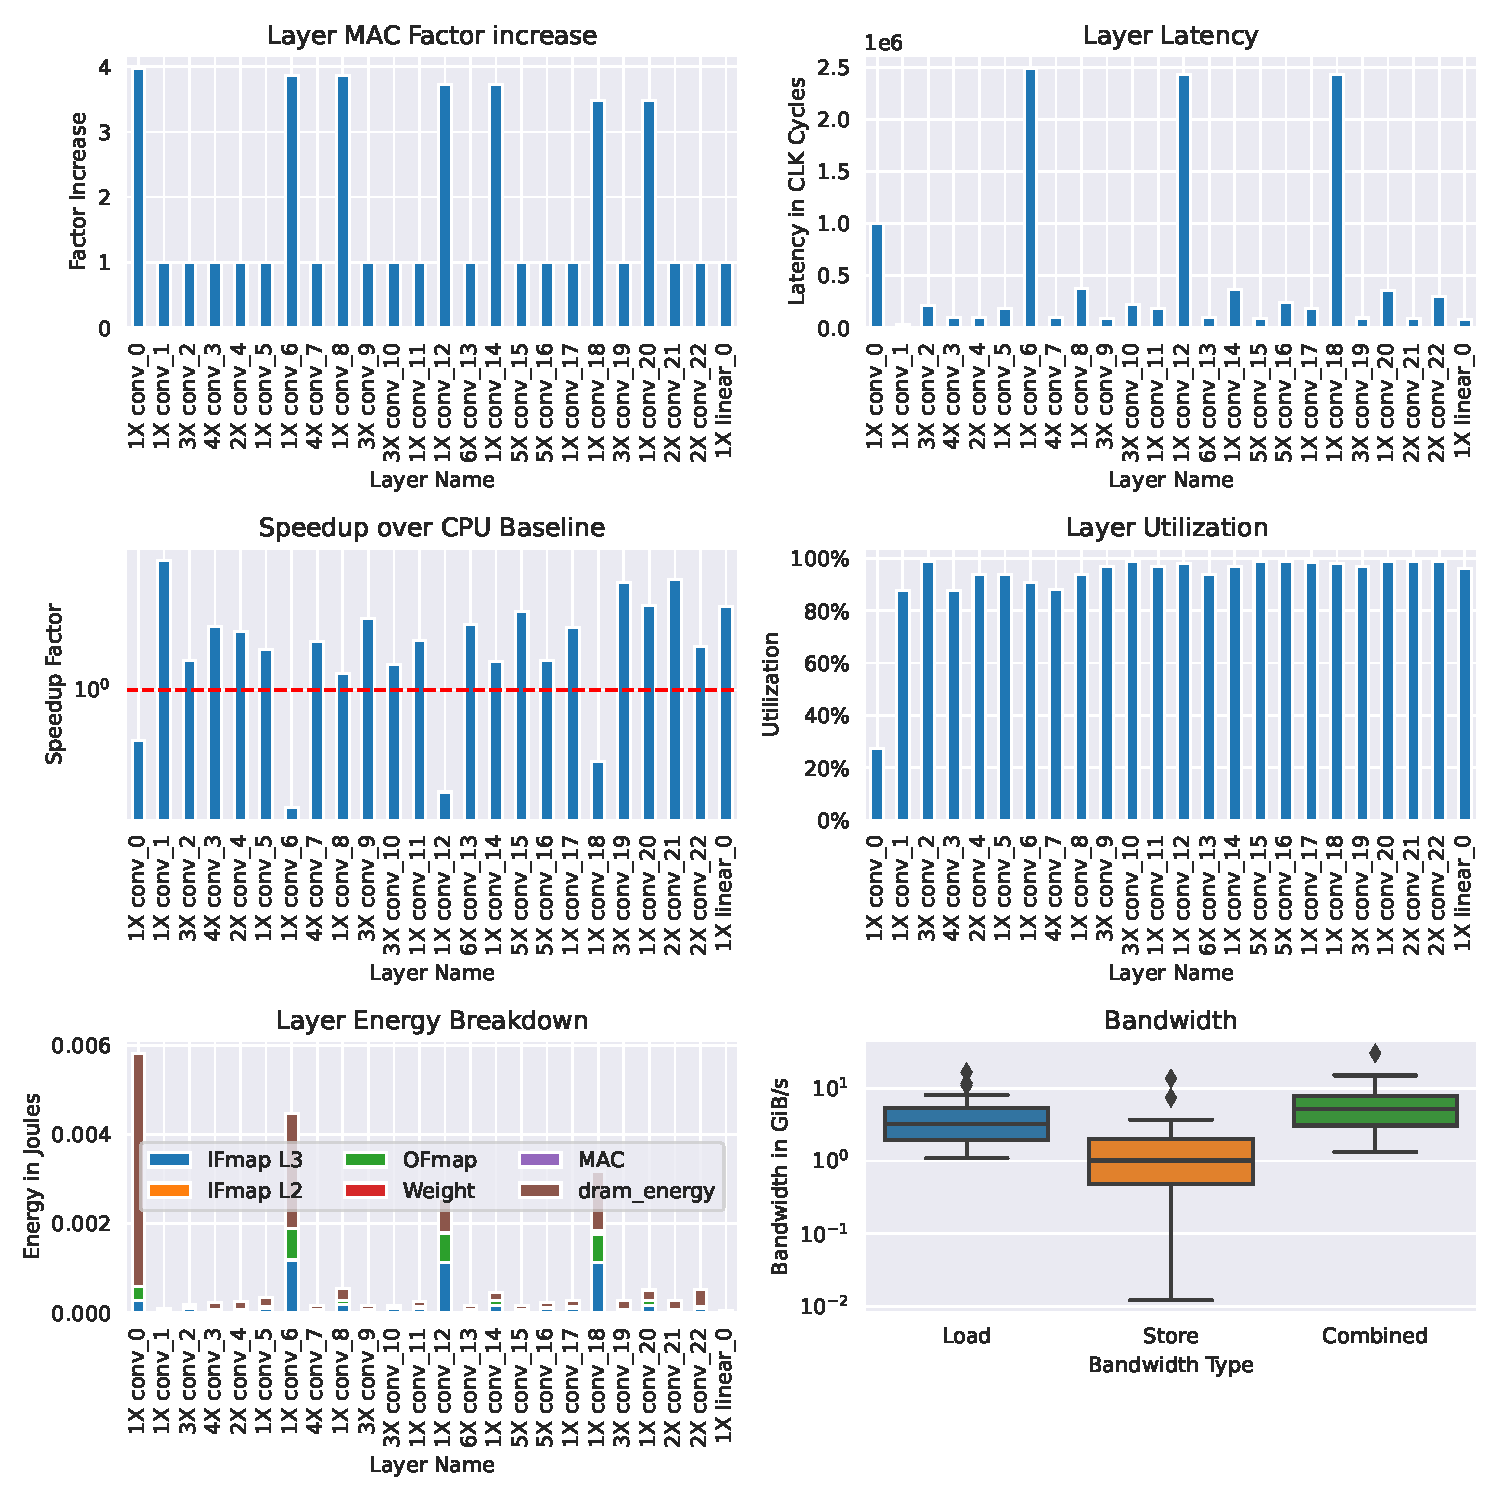
\includegraphics[scale=0.6]{Plots/networks/resnet50.pdf}
    \caption{Hardware Implementation Taxonomy adapted from \cite{maestro}}
    \label{fig:hw_taxonomy}
\end{figure}
